\documentclass[11pt]{book}
\usepackage{gvv-book}
\usepackage{gvv}
\usepackage[sectionbib,authoryear]{natbib}
\setcounter{secnumdepth}{3}
\setcounter{tocdepth}{2}
\makeindex

\begin{document}
\frontmatter
\tableofcontents
\setcounter{page}{1}
\mainmatter
\chapter{Triangle}
Consider a triangle with vertices
\begin{align}
\label{eq:tri-pts}
\vec{A}=\myvec{-3 \\ -5},\,
\vec{B}=\myvec{3\\-5},\,
	\vec{c}=\myvec{-4\\-3},\,
\end{align}

\section{Vectors}


\begin{enumerate}[label=\thesection.\arabic*.,ref=\thesection.\theenumi]
\numberwithin{equation}{enumi}

\item The direction vector of $AB$ is defined as
		\begin{align}
			\vec{B}-
			\vec{A}
		\end{align}
Consider a triangle with vertices
\begin{align} 
 \vec{A} &= \myvec{ -3\\ -5 } \\ \vec{B} &= \myvec{ 3\\ -5 }
  \\\vec{C} &= \myvec{ -4\\ -3}
 \end{align}
The Direction Vector of $AB$ is defined as 
\begin{align} 
\vec{B} - \vec{A}
\end{align}
Question1.1.1 :Find the Direction Vectors of $AB$,$BC$,$CA$.\\
\solution

\begin{enumerate} 
\item  The Direction vector of $AB$ is \begin{align} &= \vec{B} - \vec{A} \\
 &= \myvec{ 3 - (-3)\\ -5 - (-5) } \\&= \myvec{ 6\\ 0 }
 \end{align}
 
\item The Direction vector of $BC$ \begin{align}&= \vec{C} - \vec{B}\\
 &= \myvec{ -4 - (3)\\ -3 - (-5) } \\&= \myvec{-7 \\ 2 }
  \end{align}
  
  \item  The Direction vector of $CA$  \begin{align} &= \vec{A} - \vec{C} \\ 
 &= \myvec{ -3 - (-4)\\ -5 - (-3) } \\&= \myvec{ 1\\ -2 }
  \end{align}
 \end{enumerate}

\item The length of side $BC$ is 
		\begin{align}
			\norm{\vec{B}-\vec{A}} \triangleq \sqrt{\brak{\vec{B}-\vec{A}}^{\top}{\vec{B}-\vec{A}}}
		\end{align}
		where
		\begin{align}
			\vec{A}^{\top}\triangleq\myvec{-3 & -5}
		\end{align}
Question 1.1.2 : Find the length of side AB, BC, CA.\\
\solution
Solving for BC
Given, 
\begin{align}
\vec{A} = \myvec{-3\\-5},
\vec{B} = \myvec{3\\-5},
\vec{C} = \myvec{-4\\-3} \\  
 \norm{\vec{B}-\vec{C}}\ &=  \sqrt{\brak{\vec{B}-\vec{C}}^{\top}\brak{\vec{B}-\vec{C}}} \\
 \vec{B}-\vec{C} &= \myvec{3 \\ -5} - \myvec{-4 \\ -3} \\
 \vec{B}-\vec{C} &= \myvec{7 \\ -2} \\
 \brak{\vec{B}-\vec{C}}^{\top} &= {\myvec{7 \\ -2}}^{\top} = \myvec{7 \ -2} \\
\brak{\vec{B}-\vec{C}}^{\top}\brak{\vec{B}-\vec{C}} &= \myvec{7 \ -2} \myvec{7 \\ -2}\\
             &= 49+4 \\
             &= 53 \\  
 \sqrt{\brak{\vec{B}-\vec{C}}^{\top}\brak{\vec{B}-\vec{C}}} &= \sqrt{53}	\\
	\implies \norm{\vec{B}-\vec{C}}\ &= \sqrt{53} 
\end{align}

Solving for AB 
Given, 
\begin{align}  
 \norm{\vec{A}-\vec{B}}\ &=  \sqrt{\brak{\vec{A}-\vec{B}}^{\top}\brak{\vec{A}-\vec{B}}} \\
 \vec{A}-\vec{B} &= \myvec{-3 \\ -5} - \myvec{3 \\ -5} \\
 \vec{A}-\vec{B} &= \myvec{-6 \\ 0} \\
 \brak{\vec{A}-\vec{B}}^{\top} &= {\myvec{-6 \\ 0}}^{\top} = \myvec{-6 \ -0} \\
\brak{\vec{A}-\vec{B}}^{\top}\brak{\vec{A}-\vec{B}} &= \myvec{-6 \ 0} \myvec{-6 \\ 0}\\
             &= 36 + 0 \\
             &= 36 \\  
	\sqrt{\brak{\vec{A}-\vec{B}}^{\top}\brak{\vec{A}-\vec{B}}} &= \sqrt{36}	\\
	\implies \norm{\vec{A}-\vec{B}}\ &= \sqrt{36} 
\end{align}

Solving for CA
Given, 
\begin{align}  
	\norm{\vec{C}-\vec{A}}\ &=  \sqrt{\brak{\vec{C}-\vec{A}}^{\top}\brak{\vec{C}-\vec{A}}} \\
 \vec{C}-\vec{A} &= \myvec{-4 \\ -3} - \myvec{-3 \\ -5} \\
 \vec{C}-\vec{A} &= \myvec{-1 \\ 2} \\
 \brak{\vec{C}-\vec{A}}^{\top} &= {\myvec{-1 \\ 2}}^{\top} = \myvec{-1 \ 2} \\
	\brak{\vec{C}-\vec{A}}^{\top}\brak{\vec{C}-\vec{A}} &= \myvec{-1 \ 2} \myvec{-1 \\ 2}\\
             &= 1 + 4 \\
             &= 5 \\  
	\sqrt{\brak{\vec{C}-\vec{A}}^{\top}\brak{\vec{C}-\vec{A}}} &= \sqrt{5}	\\
	\implies \norm{\vec{C}-\vec{A}}\ &= \sqrt{5} 
\end{align}



\item   Points $\vec{A}, \vec{B}, \vec{C}$ are defined to be collinear if 
		\begin{align}
			\rank{\myvec{1 & 1 & 1 \\ \vec{A}& \vec{B}&\vec{C}}} = 2
		\end{align}
Are the given points in
			\eqref{eq:tri-pts}
collinear?\\
Question 1.1.3 : Check the collinearity of $\vec{A},\vec{B},\vec{C}$ \\ 
\solution 
Given that,
\begin{align}
    \vec{A} = \myvec{-3\\-5}
    \quad
    \vec{B} &= \myvec{3\\-5}
    \quad
    \vec{C} = \myvec{-4\\-3}
\end{align}
Given that $\vec{A},\vec{B},\vec{C}$ are collinear if
\begin{align}
    \text{rank}\myvec{
    1 & 1 & 1\\
    \vec{A} & \vec{B} & \vec{C} \\
    } &< 3 
    \label{eq:1.1.3,2}
\end{align} 
Let
\begin{align}
    \vec{R}&=\myvec{
    1 & 1 & 1
    \\
    -3 & 3 & -4
    \\
    -5 & -5 & -3
    } 
\end{align} 
The matrix $\vec{R}$ can be row reduced as follows,
\begin{align}
    \label{eq:matthrowoperations}
    \myvec{
    1 & 1 & 1
    \\
    -3 & 3 & -4
    \\
    -5 & -5 & -3
    }
     \xleftrightarrow[]{R_3 \leftarrow R_3+5R_1}
    \myvec{
    1 & 1 & 1
    \\
    -3 & 3 & -4
    \\
    0 & 0 & 2 
    }
    \\
     \xleftrightarrow[]{R_2\leftarrow R_2+3R_1}
    \myvec{
    1 & 1 & 1
    \\
    0 & 6 & -1
    \\
    0 & 0 & 2 
    }
\end{align}
There are no zero rows. So,
\begin{align}
    \text{rank}\myvec{
    1 & 1 & 1\\
    \vec{A} & \vec{B} & \vec{C} \\
    } &= 3 
\end{align}  
Hence, from \eqref{eq:1.1.3,2} the points $\vec{A},\vec{B},\vec{C}$ are not collinear. 

From Fig. \ref{fig1:Triangle}, We can see that $\vec{A},\vec{B},\vec{C}$ are not collinear .
\begin{figure}[h]
\centering
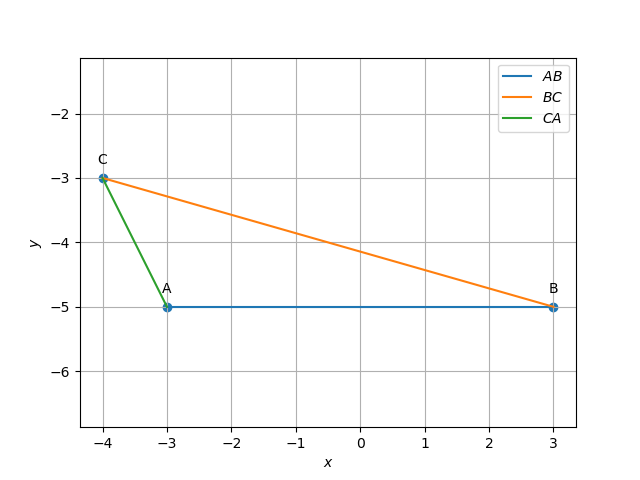
\includegraphics[width=\columnwidth]{figs/collinear.jpg}
\caption{$\vec{A},\vec{B},\vec{C}$ plot}
\label{fig1:Triangle}
\end{figure}



\item The parameteric form of the equation  of $AB$ is 
		\begin{align}
			\vec{x}=\vec{A}+k\vec{m}
		\end{align}
		where
		\begin{align}
\vec{m}=\vec{B}-\vec{A}
		\end{align}
is the direction vector of $AB$.\\
Question 1.1.4 :Find the parametric equation of $AB$,$BC$,$CA$.\\
\solution
The parametric equation for AB is given by
\begin{align}
\vec{x} &= \vec{A} + k\vec{m}\\
\text{where, } \vec{m} &= \vec{B} -\vec{A}\\
&= \myvec{3 \\ -5} -\myvec{-3\\ -5}\\
&= \myvec{6 \\0}
\end{align}
Hence we get,
\begin{align}
AB: \vec{x} = &\myvec{-3\\-5} + k \myvec{6\\0}
\end{align}
Similarly, 
\begin{align}
BC: \vec{x} = &\myvec{3\\-5} + k \myvec{-7\\2}\\
CA: \vec{x} = &\myvec{-4\\-3} + k \myvec{1\\-2}
\end{align}


\item The normal form of the equation of $AB$  is 
		\begin{align}
			\vec{n}^{\top}\brak{	\vec{x}-\vec{A}} = 0
		\end{align}
		where 
		\begin{align}
			\vec{n}^{\top}\vec{m}&=\vec{n}^{\top}\brak{\vec{B}-\vec{A}} = 0
			\\
			\text{or, } \vec{n}&=\myvec{0 & 1 \\ -1 & 0} \vec{m}
		\end{align}
  \begin{align}
\vec{n}^{\top}\myvec{\vec{x}-\vec{A}}=0
\end{align}
where
\begin{align}
\vec{n}^{\top}\vec{m}&=\vec{n}^{\top}\myvec{\vec{B}-\vec{A}}=0
\end{align}	
or,\begin{align}
\vec{n}&=\myvec{0 &1 \\-1 & 0}\vec{m}
\end{align}
Question 1.1.5:Find the normal form of the equations of $AB, BC$ and $CA$.\\
\solution:
       The normal equation for the side $AB$ is
\begin{align}
\vec{n}^{\top}\myvec{\vec{x}-\vec{A}}&=0\\
\implies
\vec{n}^{\top}\vec{x}&=\vec{n}^{\top}\vec{A}
\end{align}
Now our task is to find the $\vec{n}$ so that we can find $\vec{n}^{\top}$.
As given in the question 
\begin{align}
  \vec{n} &= \myvec{0 & 1\\
  -1 & 0}\vec{m}
\end{align}
Here $\vec{m} = \vec{B}- \vec{A}$ for side $\vec{AB}$
\begin{align}
\implies
\vec{m}&=\myvec{3\\-5} - \myvec{-3\\-5}\\
&=\myvec{6\\0}
\end{align}
Now as we have obtained vector $\vec{m}$.
we can use this to obtain vector $\vec{n}$
\begin{align}
\vec{n} &= \myvec{0 & 1\\
  -1 & 0}\myvec{6\\0}
 = \myvec{0\\-6}
\end{align}
The transpose of $\vec{n}$ is
\begin{align}
  \vec{n}^{\top}&=\myvec{0 & -6}
\end{align}
Hence the normal equation of side $AB$ is 
\begin{align}
    \myvec{0 & -6}\vec{x}&=\myvec{0 & -6}\myvec{-3\\-5}\\
    \implies
    \myvec{0 & -6}\vec{x}&=30
\end{align}
\begin{figure}
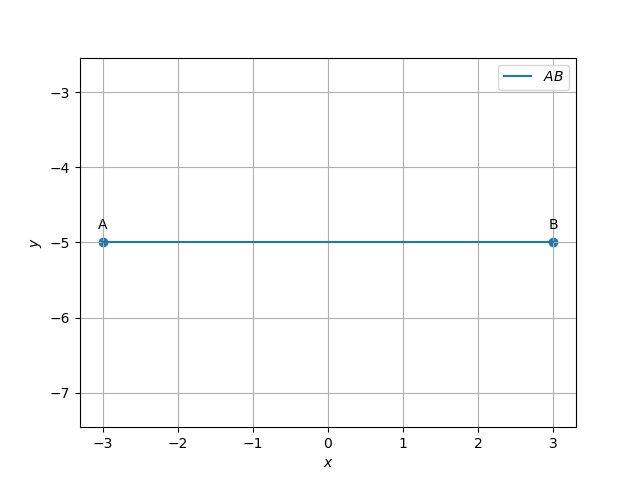
\includegraphics [width=\columnwidth] {figs/lineab.png}
\caption{ The line $\vec{AB}$ plotted using python}
\label{fig: lineab}
\end{figure}


       The normal equation for the side $BC$ is
\begin{align}
\vec{n}^{\top}\myvec{\vec{x}-\vec{B}}&=0\\
\implies
\vec{n}^{\top}\vec{x}&=\vec{n}^{\top}\vec{B}
\end{align}
Now our task is to find the $\vec{n}$ so that we can find $\vec{n}^{\top}$.
As given in the question 
\begin{align}
  \vec{n} &= \myvec{0 & 1\\
  -1 & 0}\vec{m}
\end{align}
Here $\vec{m} = \vec{C}- \vec{B}$ for side $\vec{BC}$
\begin{align}
\implies
\vec{m}&=\myvec{-4\\-3} - \myvec{3\\-5}\\
&=\myvec{-7\\2}
\end{align}
Now as we have obtained vector $\vec{m}$.
we can use this to obtain vector $\vec{n}$
\begin{align}
\vec{n} &= \myvec{0 & 1\\
  -1 & 0}\myvec{-7\\2}
 = \myvec{2\\7}
\end{align}
The transpose of $\vec{n}$ is
\begin{align}
  \vec{n}^{\top}&=\myvec{2 & 7}
\end{align}
Hence the normal equation of side $BC$ is 
\begin{align}
    \myvec{2 & 7}\vec{x}&=\myvec{2 & 7}\myvec{3\\-5}\\
    \implies
    \myvec{2 & 7}\vec{x}&=-29
\end{align}
\begin{figure}
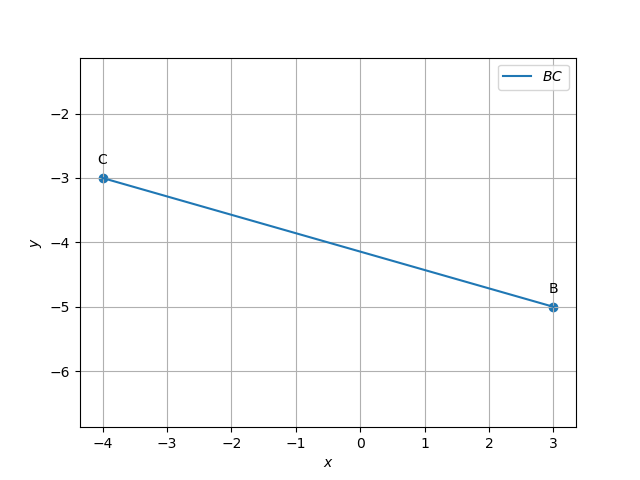
\includegraphics [width=\columnwidth] {figs/linebc.png}
\caption{ The line $\vec{BC}$ plotted using python}
\label{fig: linebc}
\end{figure}



       The normal equation for the side $CA$ is
\begin{align}
\vec{n}^{\top}\myvec{\vec{x}-\vec{C}}&=0\\
\implies
\vec{n}^{\top}\vec{x}&=\vec{n}^{\top}\vec{C}
\end{align}
Now our task is to find the $\vec{n}$ so that we can find $\vec{n}^{\top}$.
As given in the question 
\begin{align}
  \vec{n} &= \myvec{0 & 1\\
  -1 & 0}\vec{m}
\end{align}
Here $\vec{m} = \vec{A}- \vec{C}$ for side $\vec{CA}$
\begin{align}
\implies
\vec{m}&=\myvec{-3\\-5} - \myvec{-4\\-3}\\
&=\myvec{1\\-2}
\end{align}
Now as we have obtained vector $\vec{m}$.
we can use this to obtain vector $\vec{n}$
\begin{align}
\vec{n} &= \myvec{0 & 1\\
  -1 & 0}\myvec{1\\-2}
 = \myvec{-2\\-1}
\end{align}
The transpose of $\vec{n}$ is
\begin{align}
  \vec{n}^{\top}&=\myvec{-2 & -1}
\end{align}
Hence the normal equation of side $CA$ is 
\begin{align}
    \myvec{-2 & -1}\vec{x}&=\myvec{-2 & -1}\myvec{-4\\-3}\\
    \implies
    \myvec{-2 & -1}\vec{x}&=11
\end{align}
\begin{figure}
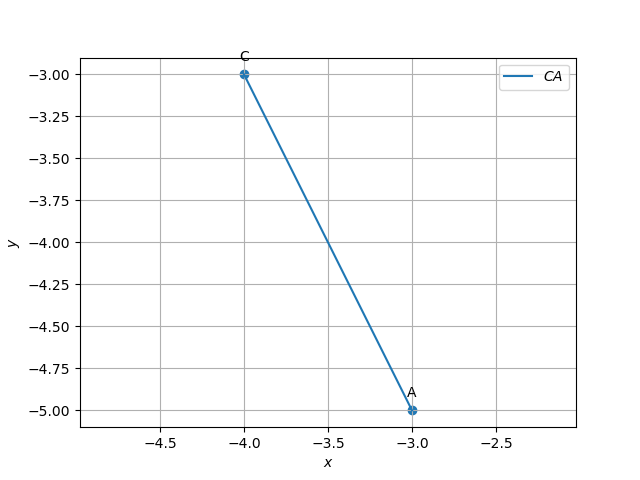
\includegraphics [width=\columnwidth] {figs/lineca.png}
\caption{ The line $\vec{CA}$ plotted using python}
\label{fig: lineca}
\end{figure}


\item The area of $\triangle ABC$ is defined as
		\begin{align}
			\frac{1}{2}\norm{{\brak{\vec{A}-\vec{B}}\times {\vec{A}-\vec{C}}}}
		\end{align}
		where
		\begin{align}
			\vec{A}\times\vec{B} \triangleq \mydet{1 & -4 \\-1 & 6}
		\end{align}
Question 1.1.6:Find the area of $\triangle$ ABC.\\
\solution
Given,
\begin{align}
\vec{A} = \myvec{-3\\-5};
\vec{B} = \myvec{3\\-5};
\vec{C} = \myvec{-4\\-3}\\
\vec{A}-\vec{B}=\myvec{-3\\-5}-\myvec{3\\-5}&=\myvec{-6\\0}\\
\vec{A}-\vec{C}=\myvec{-3\\-5}-\myvec{-4\\-3}&=\myvec{1\\-2}\\
\therefore(\vec{A}-\vec{B})\times(\vec{A}-\vec{C}) &=\mydet{-6 & 1\\0 & -2}\\
	&=(-6)\times (-2)- 1\times0\\&=12-0\\&=12\\
\implies\frac{1}{2}\norm{(\vec{A}-\vec{B})\times(\vec{A}-\vec{C})}&=\frac{12}{2}=6
\end{align}


\item
Question 1.1.7:Find the angles $\vec{A},\vec{B},\vec{C}$, given that 
\begin{align}
	\cos{A} \triangleq \frac{(\vec{B}-\vec{A})\top(\vec{C}-\vec{A})}{\norm{\vec{B}-\vec{A}}\norm{\vec{C}-\vec{A}}}
\end{align}
\solution 
\\
From the given values of $\vec{A},\vec{B},\vec{C}$,\\
\begin{enumerate}

\item Finding the value of angle A
\begin{align}
	\vec{B}-\vec{A} &=\myvec{6\\0}
\end{align}
and 
\begin{align}
	\vec{C}-\vec{A}&= \myvec{-1\\+2}
\end{align}
also calculating the values of norms
\begin{align}
	\norm{\vec{B}-\vec{A}} &= \sqrt{36} &= 6\\
	\norm{\vec{C}-\vec{A}} &= \sqrt{5}
\end{align}
and by doing matrix multiplication we get,
\begin{align}
\begin{split}
	(\vec{B}-\vec{A})^{\top}(\vec{C}-\vec{A})&=\myvec{6&0}\myvec{-1\\+2}\\
	&=-6
\end{split}
\end{align}
so 
\begin{align}
	\cos{A}&= \frac{-6}{6 \sqrt{5}}\\
	&= \frac{-1}{\sqrt{5}}\\
	\implies A&=\cos^{-1}{\frac{-1}{\sqrt{5}}}
\end{align}




\item Finding the value of angle B
\begin{align}
	\vec{C}-\vec{B} &=\myvec{-7\\2}
\end{align}
and 
\begin{align}
	\vec{A}-\vec{B}&= \myvec{-6\\0}
\end{align}
also calculating the values of norms
\begin{align}
	\norm{\vec{C}-\vec{B}} &= \sqrt{5}\\
	\norm{\vec{A}-\vec{B}} &= \sqrt{53}
\end{align}
and by doing matrix multiplication we get,
\begin{align}
\begin{split}
	(\vec{C}-\vec{B})^{\top}(\vec{A}-\vec{B})&=\myvec{-7&2}\myvec{-6\\0}\\
	&= 42
\end{split}
\end{align}
so 
\begin{align}
	\cos{B}&= \frac{42}{\sqrt{36} \sqrt{53}}\\
	&= \frac{7}{\sqrt{53}}\\
	\implies B&=\cos^{-1}{\frac{7}{\sqrt{53}}}
\end{align}



\item Finding the value of angle C
\begin{align}
	\vec{A}-\vec{C} &=\myvec{1\\-2}
\end{align}
and 
\begin{align}
	\vec{B}-\vec{C}&= \myvec{7\\-2}
\end{align}
also calculating the values of norms
\begin{align}
	\norm{\vec{A}-\vec{C}} &= \sqrt{5}\\
	\norm{\vec{B}-\vec{C}} &= \sqrt{53}
\end{align}
and by doing matrix multiplication we get,
\begin{align}
\begin{split}
	(\vec{A}-\vec{C})^{\top}(\vec{B}-\vec{C})&=\myvec{1&-2}\myvec{7\\-2}\\
	&=11
\end{split}
\end{align}
so 
\begin{align}
	\cos{C}&= \frac{11}{\sqrt{5} \sqrt{53}}\\
	&= \frac{11}{\sqrt{265}}\\
	\implies C&=\cos^{-1}{\frac{11}{\sqrt{265}}}
\end{align}

\end{enumerate}


\end{enumerate}









%\section{Median}
%\input{subsec/median}
%\section{Altitude}
%\section{Perpendicular Bisector}
%\section{Angle Bisector}

\end{document}
